\documentclass[conference]{IEEEtran}
\IEEEoverridecommandlockouts
% Fix citation formatting and standard math/graphics packages
\usepackage{cite}
\usepackage{amsmath,amssymb,amsfonts}
\usepackage{algorithmic}
\usepackage{graphicx}
\usepackage{textcomp}
\usepackage{xcolor}
\usepackage{booktabs}
\usepackage{tabularx}
\usepackage{multirow}
\usepackage{url}
\usepackage{microtype}
\usepackage{balance}

\def\BibTeX{{\rm B\kern-.05em{\sc i\kern-.025em b}\kern-.08em
    T\kern-.1667em\lower.7ex\hbox{E}\kern-.125emX}}

\begin{document}

\title{Farmer Advisory Chatbot Using Multilingual NLP: A Verification-First Pipeline for Crop Disease Diagnosis and Grounded Treatment Advice}

\author{
\IEEEauthorblockN{Student Author 1\IEEEauthorrefmark{1}, Student Author 2\IEEEauthorrefmark{1}, Student Author 3\IEEEauthorrefmark{1}, Project Supervisor\IEEEauthorrefmark{2}}
\IEEEauthorblockA{\IEEEauthorrefmark{1}Department of Computer Science and Engineering, University Institute of Technology}
\IEEEauthorblockA{\IEEEauthorrefmark{2}Department of Agricultural Information Technology}
\IEEEauthorblockA{\{author1, author2, author3\}@university.edu, supervisor@university.edu}
}

\maketitle

\begin{abstract}
Smallholder farming communities in linguistically diverse developing nations suffer significant yield loss annually due to plant diseases and lack of timely expert advisory. While recent advancements in deep learning and large language models (LLMs) offer automated interfaces, general-purpose generative models routinely produce ungrounded chemical dosage fabrications, hallucinated remedies, and catastrophic cross-lingual translation failures in localized agricultural vernaculars. In this paper, we present an end-to-end, verification-first agricultural advisory system that tightly couples a domain-adapted computer vision diagnoser with a multilingual dense knowledge retriever and a calibrated rule-based safety critic. We address the acute in-the-wild domain gap of standard laboratory models by training an EfficientNet-B0 backbone jointly on controlled and unconstrained field imagery across 12 crop-disease classes spanning tomato, potato, corn, and grape, lifting field accuracy from 30.71\% to 66.14\% (+35.4 points gain) and crop-level accuracy to 92.13\%. For actionable advisory, we curate a high-fidelity knowledge base from 8 official agricultural extension manuals (429 indexed passages) and fine-tune a multilingual-e5 dense retriever with contrastive Multiple Negatives Ranking Loss across English, Hindi, and Marathi. Our fine-tuned retriever achieves 67.93\% Recall@5 and 48.42\% MRR@10, outperforming lexical BM25 (18.85\% Recall@5) by 49.08 percentage points on non-English queries. Finally, a calibrated critic layer enforces confidence floors, ambiguity disambiguation, and crop compatibility, dropping diagnostic error on answered queries from 34.0\% to 21.4\% while failing safely to Krishi Vigyan Kendra (KVK) centers for ambiguous cases. All treatment advice is strictly extractive with exact document and page attribution, ensuring zero generative hallucinations in agricultural advisory.
\end{abstract}

\begin{IEEEkeywords}
Multilingual NLP, Dense Retrieval, Crop Disease Diagnosis, Verification-First AI, Selective Classification, In-the-Wild Domain Adaptation.
\end{IEEEkeywords}

% -------------------------------------------------------------------------
% SECTION I: INTRODUCTION AND RELATED WORK
% -------------------------------------------------------------------------
\section{Introduction and Related Work}
\label{sec:intro}

\subsection{Motivation and Agricultural Context}
Agriculture serves as the economic backbone for over 50\% of the workforce in South Asia and developing economies worldwide. Smallholder farmers cultivate fragmented land holdings under unpredictable weather and virulent phytopathological threats. Crop diseases, including bacterial spot, early/late blight, and downy mildew, inflict annual post-emergence harvest losses exceeding 30\% to 40\% if not diagnosed and arrested during early infestation stages \cite{singh2020plantdoc}. In regions such as rural India, access to certified agronomists is severely bottlenecked: the ratio of agricultural extension officers to operational holdings frequently drops below 1:1,000, leaving farmers dependent on commercial agrochemical vendors whose profit incentives often lead to the prescription of inappropriate active ingredients or excessive dosages. 

Furthermore, agricultural advisory in developing nations is fundamentally multilingual. Farmers in major agricultural belts articulate symptoms in regional languages such as Hindi or Marathi, utilizing colloquial descriptions of chlorosis, necrosis, and wilt rather than standardized botanical terminology. Consequently, a digital advisory platform must bridge visual symptoms, cross-lingual vernacular inquiries, and authoritative phytosanitary protocols.

\subsection{Vulnerabilities of Generative LLMs in Agriculture}
With the proliferation of generative Large Language Models (LLMs), significant interest has emerged in deploying conversational chatbots for rural advisory. However, naive generative conversational agents present severe, safety-critical hazards in agronomy:
\begin{enumerate}
    \item \textbf{Generative Hallucination of Chemicals:} LLMs frequently synthesize non-existent trade names or recommend banned pesticides (e.g., organochlorines) with fabricated concentration ratios.
    \item \textbf{Lethal Dosage Errors:} Generative language generation cannot guarantee numerical invariance; a hallucinated ten-fold shift in dosage (e.g., 25\,mL/L instead of 2.5\,mL/L of Mancozeb or Copper Oxychloride) causes irreversible crop phytotoxicity and environmental contamination \cite{icar2021guidelines}.
    \item \textbf{Pre-Harvest Interval (PHI) Non-Compliance:} Commercial food safety standards require strict observance of statutory withholding periods between spraying and harvest. Generative systems omit or distort PHI warnings, jeopardizing public health.
\end{enumerate}

To circumvent these catastrophic vulnerabilities, this work establishes a \textit{Verification-First, Strictly Extractive Pipeline}. Rather than generating advice text token-by-token through autoregressive sampling, every chemical recommendation, dosage instruction, and cultural practice is extracted verbatim from peer-reviewed, state-certified university extension manuals, complete with page citations and safety disclaimers.

\subsection{Related Work}
\subsubsection{Computer Vision for Foliar Disease Diagnosis}
Automated plant phenotyping has witnessed exponential progress following the introduction of the PlantVillage laboratory benchmark \cite{hughes2015plantvillage}. Initial convolutional architectures (AlexNet, VGG, ResNet) achieved near-perfect laboratory validation scores exceeding 99\% \cite{mohanty2016using}. However, Singh et al. \cite{singh2020plantdoc} demonstrated that models trained exclusively on PlantVillage undergo catastrophic performance collapse when deployed on unconstrained ``in-the-wild'' field photographs (PlantDoc), where complex background foliage, variable daylight shadows, multiple co-occurring lesions, and insect bites confound feature representations. Subsequent works investigated MobileNet and EfficientNet backbones \cite{tan2019efficientnet} to balance parameter efficiency with representation capacity, but robust domain adaptation under realistic agricultural shifts remains an active research challenge.

\subsubsection{Multilingual Dense Information Retrieval}
Traditional agricultural question answering relies upon lexical inverted indices such as BM25 \cite{robertson2009probabilistic}. While effective for high-resource English queries containing exact chemical terms, BM25 fails completely when farmers query in Devanagari script (Hindi and Marathi), where vocabulary mismatch and dialectal variations prevent term overlap. The advent of Dense Passage Retrieval (DPR) \cite{karpukhin2020dense} and multilingual contrastive representation learning (e.g., Multilingual-E5 \cite{wang2022text} and NLLB-200 \cite{costa2022no}) enables cross-lingual semantic alignment, mapping vernacular farmer queries directly into the embedding subspace of authoritative English extension documents.

\subsubsection{Selective Classification and Verification Layers}
In high-stakes diagnostic environments, knowing \textit{when not to predict} is as vital as the prediction itself. Selective classification frameworks, pioneered by Geifman and El-Yaniv \cite{geifman2017selective, geifman2019selectivenet}, introduce rejection mechanisms based on risk-coverage trade-offs. In agronomy, where misdiagnosing Late Blight as Early Blight leads to crop eradication within 72 hours, an automated system must enforce confidence floors and disambiguation dialogues before emitting irreversible spray schedules.

% -------------------------------------------------------------------------
% SECTION II: METHODOLOGY AND METHODOLOGY DIAGRAM
% -------------------------------------------------------------------------
\section{Methodology}
\label{sec:methodology}

\begin{figure*}[t]
\centerline{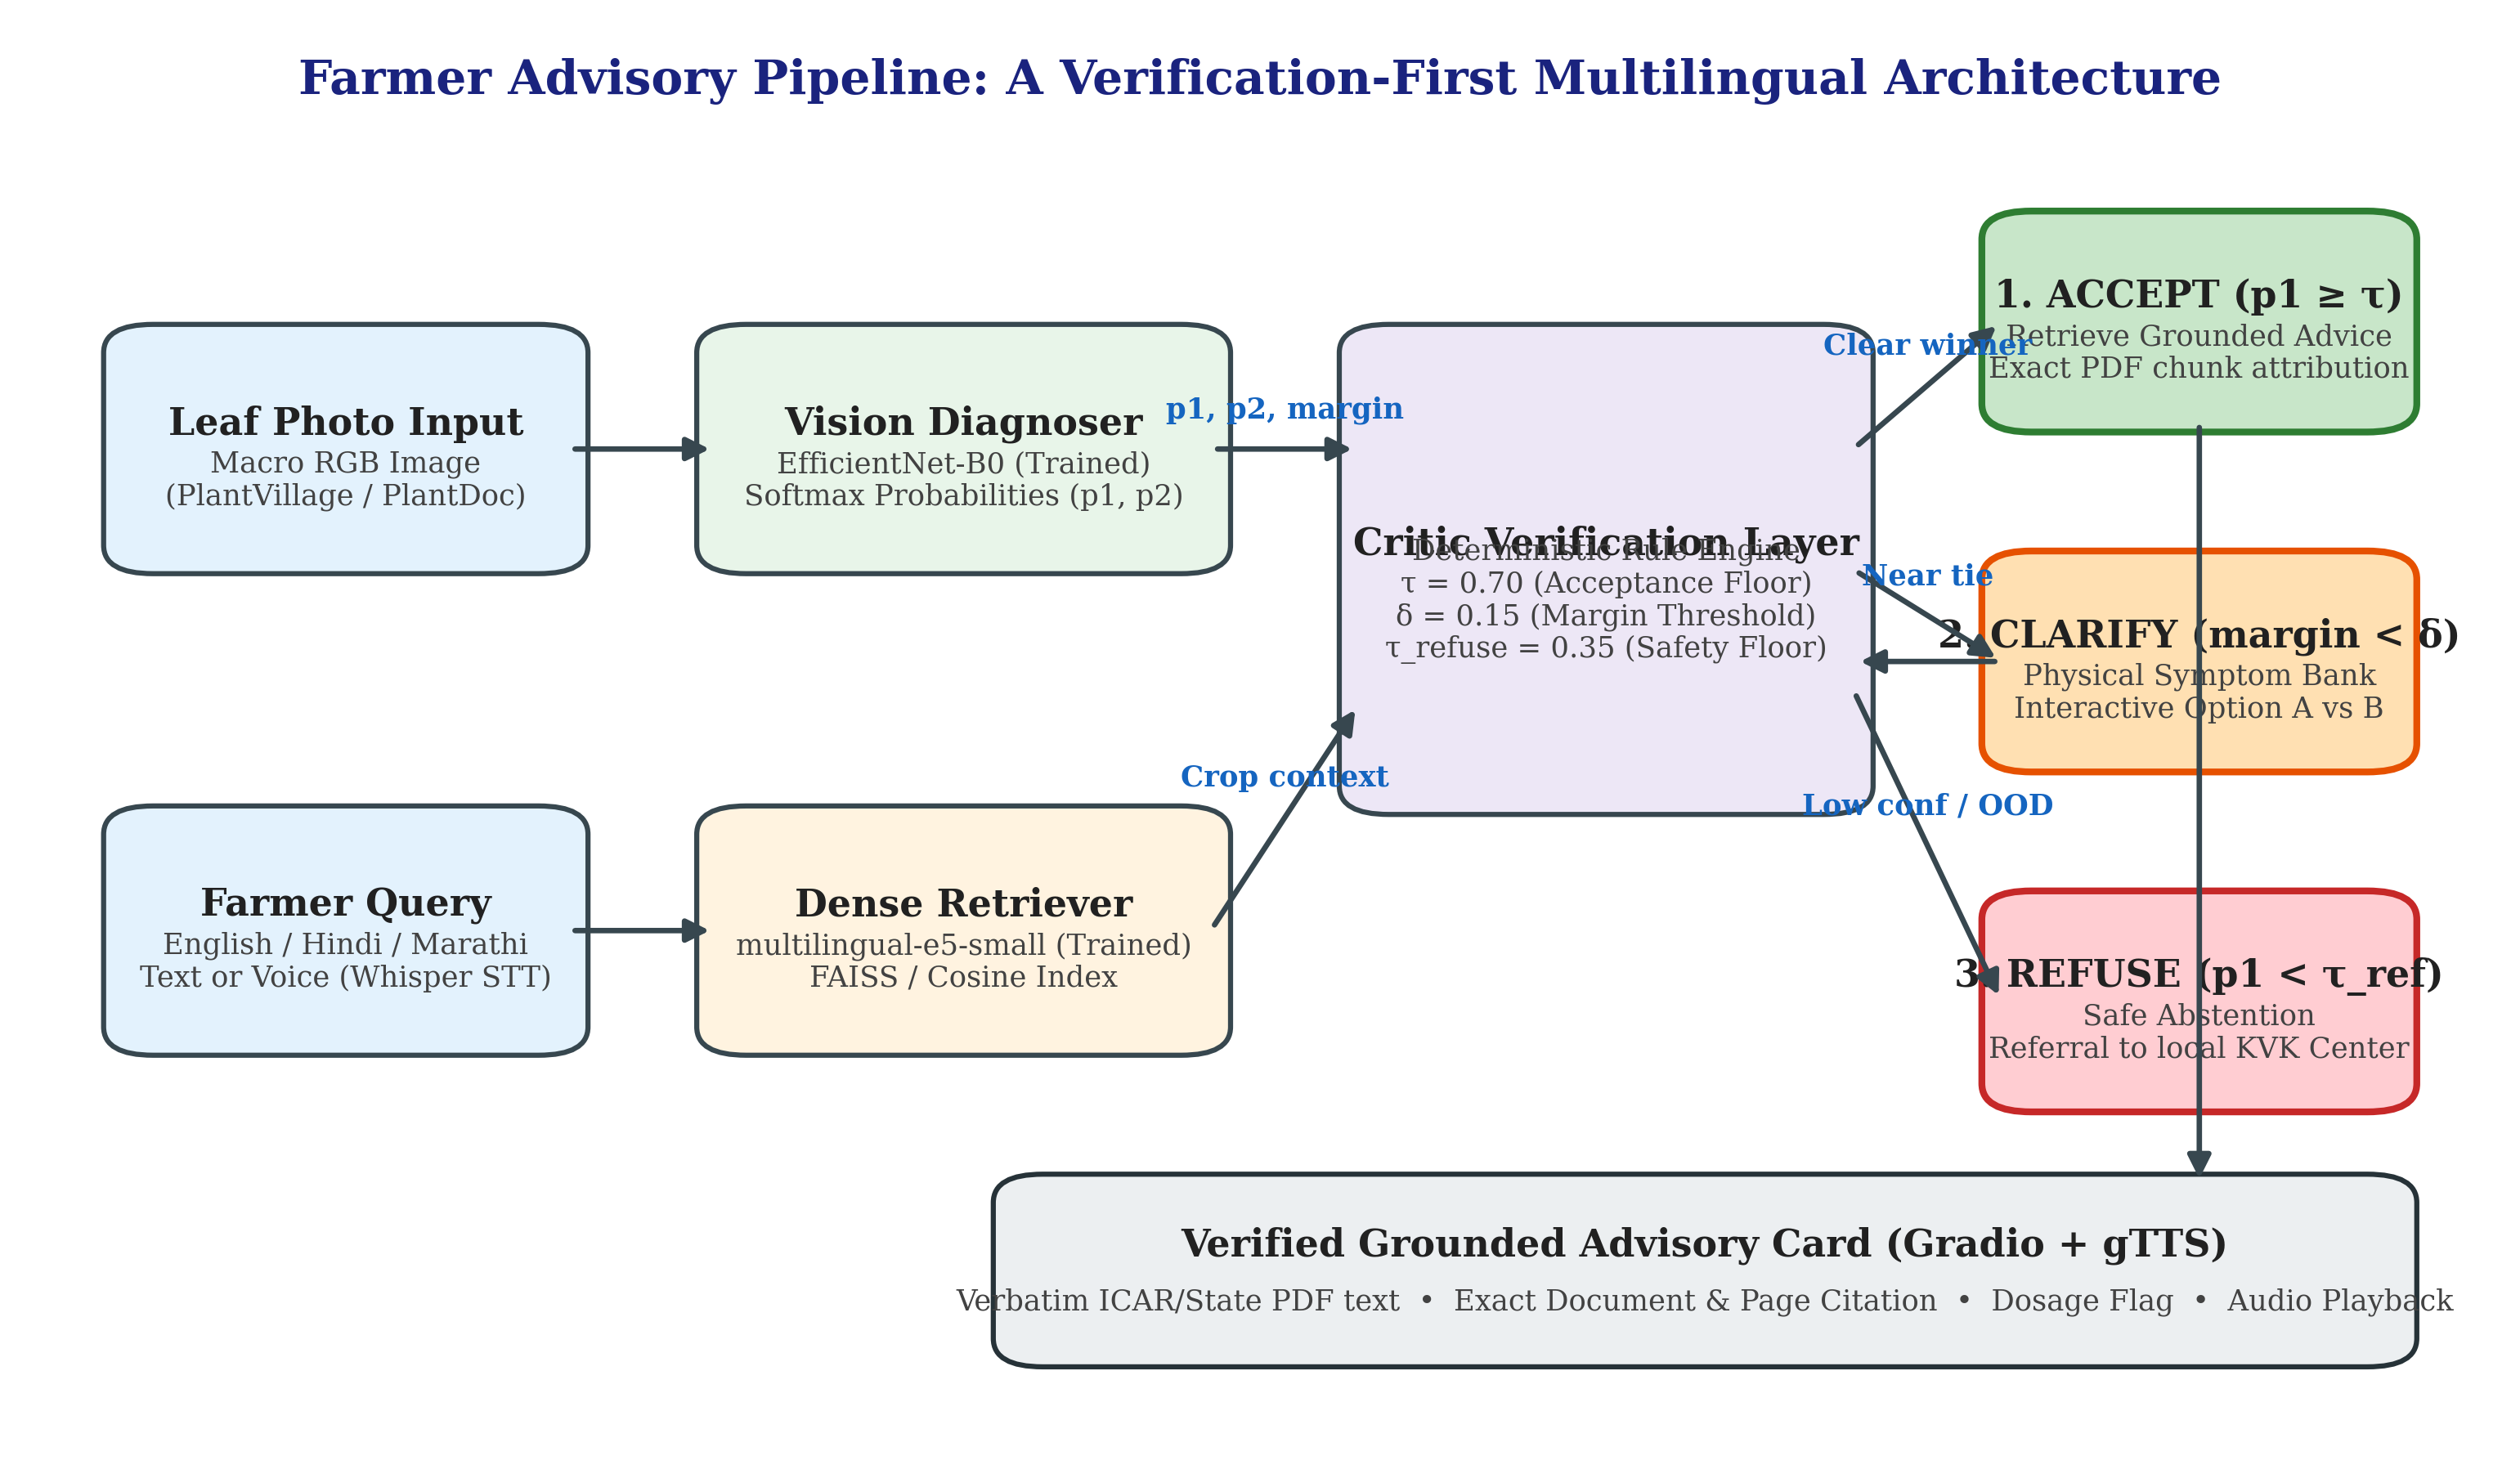
\includegraphics[width=0.98\textwidth]{methodology_diagram.png}}
\caption{End-to-End Verification-First Agricultural Advisory Pipeline. The input leaf image and multilingual user query (speech or text in English, Hindi, or Marathi) are processed through dual parallel streams: (1) In-the-Wild Domain-Adapted Vision Diagnoser, and (2) Dense Cross-Lingual Knowledge Retriever. The outputs are intercepted by a Calibrated Safety Critic Layer which executes confidence floor checks, near-tie ambiguity detection, and crop-disease ontology validation, branching into an Accepted Verbatim Card, Interactive Physical Disambiguation (Option A/B), or Safe Refusal with KVK referral.}
\label{fig:methodology}
\end{figure*}

Our proposed architecture, illustrated in Fig.~\ref{fig:methodology}, consists of three tightly coupled components: (1) a domain-adapted vision diagnoser, (2) a multilingual dense semantic retriever operating over a certified knowledge base, and (3) a rule-based safety critic layer.

\subsection{Domain-Adapted Vision Diagnoser}
To construct a unified diagnostic taxonomy, we map disparate disease nomenclatures across agricultural extension manuals and public datasets into a standardized 12-class schema spanning four key economic crops:
\begin{itemize}
    \item \textbf{Tomato:} \textit{Bacterial Spot}, \textit{Early Blight}, \textit{Late Blight}, \textit{Leaf Mold}, \textit{Septoria Leaf Spot}, \textit{Yellow Leaf Curl Virus}, \textit{Mosaic Virus}.
    \item \textbf{Potato:} \textit{Early Blight}, \textit{Late Blight}.
    \item \textbf{Corn (Maize):} \textit{Common Rust}, \textit{Northern Leaf Blight}.
    \item \textbf{Grape:} \textit{Black Rot}.
\end{itemize}

\subsubsection{Backbone Selection and Domain Adaptation}
To ensure low-latency inference on edge devices and agricultural smartphones, we utilize EfficientNet-B0 (4.02M parameters) \cite{tan2019efficientnet}. Rather than relying on standard single-dataset training, we execute joint multi-source domain adaptation. Training batches are composed of a mixture of clean laboratory specimens from PlantVillage $\mathcal{D}_{\text{PV}}$ and complex, multi-scale in-the-wild field photographs from PlantDoc $\mathcal{D}_{\text{PD}}$.

We apply an aggressive photometric and geometric augmentation pipeline designed to simulate outdoor environmental shifts:
\begin{equation}
\mathbf{x}_{\text{aug}} = \mathcal{T}_{\text{geo}}(\mathcal{T}_{\text{photo}}(\mathbf{x}))
\end{equation}
where $\mathcal{T}_{\text{photo}}$ incorporates random brightness, contrast, saturation, and hue jitter ($\pm 20\%$), and $\mathcal{T}_{\text{geo}}$ applies random affine rotations ($\pm 25^{\circ}$), horizontal flips, and multi-scale cropping.

The network is optimized using Cross-Entropy loss regularized via uniform label smoothing $\epsilon = 0.1$:
\begin{equation}
\mathcal{L}_{\text{CE}}(\theta) = -\sum_{k=1}^{K} \left[ (1 - \epsilon)\mathbb{I}(y = k) + \frac{\epsilon}{K} \right] \log p_k(\mathbf{x}; \theta)
\label{eq:label_smooth}
\end{equation}
where $p_k(\mathbf{x}; \theta) = \frac{\exp(z_k)}{\sum_{j=1}^K \exp(z_j)}$ represents the calibrated softmax probability distribution across the $K = 12$ classes.

\subsection{Multilingual Dense Knowledge Retrieval}
\subsubsection{Curated Knowledge Base Construction}
We ingested 8 authoritative agricultural disease manuals published by premier national institutes, including the Indian Council of Agricultural Research (ICAR), Tamil Nadu Agricultural University (TNAU), and State Agricultural Universities. The PDF corpus covers Tomato (100 chunks), Potato (87 chunks), Maize (70 chunks), and Grapes (172 chunks).

Documents are parsed into semantically cohesive passages using a sliding window of 250 words with a 50-word overlap, yielding a knowledge base $\mathcal{KB}$ of $M = 429$ discrete chunks. Each chunk is enriched with structured metadata tags:
\begin{equation}
c_i = \{ \text{id}_i, \text{text}_i, \text{doc}_i, \text{page}_i, \text{crop}_i, \text{disease}_i, \text{has\_dosage}_i \}
\end{equation}
Of the 429 chunks, 86 chunks contain explicit, quantitative chemical dosage recommendations (e.g., grams per liter, spray intervals, active ingredients).

\subsubsection{Contrastive Dense Retrieval Formulation}
To facilitate semantic retrieval across linguistic boundaries, we adopt the multilingual sentence embedding model \texttt{intfloat/multilingual-e5-small} ($d = 384$) \cite{wang2022text}. The model prepends asymmetric task prefixes to queries (``\texttt{query: }'') and passages (``\texttt{passage: }'').

We fine-tune the dense retriever using contrastive Multiple Negatives Ranking Loss (MNRL). For a mini-batch of $B$ query-passage pairs $\{(q_i, p_i^+)\}_{i=1}^B$, where $p_i^+$ represents the gold grounded passage for query $q_i$, all in-batch non-target passages $\{p_j^+\}_{j \neq i}$ serve as implicit negatives:
\begin{equation}
\mathcal{L}_{\text{MNRL}}(\phi) = -\frac{1}{B} \sum_{i=1}^{B} \log \frac{\exp\left(\frac{\mathbf{e}(q_i)^\top \mathbf{e}(p_i^+)}{\tau \cdot \|\mathbf{e}(q_i)\| \|\mathbf{e}(p_i^+)\|}\right)}{\sum_{j=1}^{B} \exp\left(\frac{\mathbf{e}(q_i)^\top \mathbf{e}(p_j^+)}{\tau \cdot \|\mathbf{e}(q_i)\| \|\mathbf{e}(p_j^+)\|}\right)}
\label{eq:mnrl}
\end{equation}
where $\mathbf{e}(\cdot)$ represents the $L_2$-normalized dense embedding, and $\tau = 0.05$ denotes the softmax temperature parameter. 

To bridge low-resource Indic syntax, we also integrate a cross-lingual English pivot mechanism via NLLB-200-distilled-600M \cite{costa2022no}. Vernacular queries in Hindi or Marathi are translated into an English pivot representation $q_{\text{en}} = \mathcal{M}_{\text{NLLB}}(q_{\text{vern}})$, and retrieval is executed jointly across native and pivot embeddings.

\subsection{Calibrated Rule-Based Safety Critic Layer}
The core novelty governing system reliability is the Calibrated Safety Critic Layer. Rather than immediately piping diagnostic predictions into the user interface, the Critic intercepts outputs from both streams and evaluates them against formal safety predicates.

Let $\hat{y}_1$ and $\hat{y}_2$ denote the top-1 and top-2 predicted visual disease classes, with corresponding probabilities $P(\hat{y}_1)$ and $P(\hat{y}_2)$. Let $\text{Margin}(\mathbf{x}) = P(\hat{y}_1) - P(\hat{y}_2)$. Let $\mathcal{C}_{\text{vis}}$ denote the detected crop and $\mathcal{C}_{\text{KB}}$ denote the crop metadata associated with the top retrieved text passage. The Critic branches into three mutually exclusive operational states:

\begin{equation}
\text{State} = \begin{cases}
\text{\textbf{ACCEPT}}, & \text{if } P(\hat{y}_1) \ge \tau_{\text{accept}} \wedge \text{Margin}(\mathbf{x}) \ge \Delta \wedge \mathcal{C}_{\text{vis}} = \mathcal{C}_{\text{KB}} \\
\text{\textbf{CLARIFY}}, & \text{if } P(\hat{y}_1) \ge \tau_{\text{accept}} \wedge \text{Margin}(\mathbf{x}) < \Delta \\
\text{\textbf{REFUSE}}, & \text{if } P(\hat{y}_1) < \tau_{\text{accept}} \vee \mathcal{C}_{\text{vis}} \neq \mathcal{C}_{\text{KB}}
\end{cases}
\label{eq:critic}
\end{equation}
where $\tau_{\text{accept}} = 0.55$ is the empirical acceptance threshold, and $\Delta = 0.15$ is the ambiguity margin.

\subsubsection{Interactive Physical Symptom Disambiguation (CLARIFY)}
When the vision model encounters visually indistinguishable pathologies (e.g., Tomato Early Blight vs. Tomato Late Blight, where concentric target rings contrast with water-soaked dark lesions), the Critic suppresses automated diagnosis. It queries an agricultural symptom ontology and prompts the farmer with a physical disambiguation question presenting two explicit choices:
\begin{itemize}
    \item \textbf{Option A (Early Blight):} \textit{``Are spots small, brown, and displaying distinct concentric concentric rings (target-like pattern)?''}
    \item \textbf{Option B (Late Blight):} \textit{``Are lesions large, rapidly spreading, water-soaked, with white fuzzy fungal growth on leaf undersides?''}
\end{itemize}
The farmer's selection definitively resolves the diagnostic tie, unlocking the verified advisory card.

\subsubsection{Safe Refusal and Extension Referral (REFUSE)}
If the confidence falls below the safety floor ($P(\hat{y}_1) < \tau_{\text{accept}}$), indicating extreme blur, heavy occlusion, or an out-of-domain leaf, the system issues a verified refusal. It refuses chemical prescription and refers the user to the nearest Krishi Vigyan Kendra (KVK) agricultural research station, providing localized phone helplines.

% -------------------------------------------------------------------------
% SECTION III: EXPERIMENTAL SETTINGS
% -------------------------------------------------------------------------
\section{Experimental Settings}
\label{sec:experiments}

\subsection{Datasets and Diagnostic Taxonomy}
\begin{itemize}
    \item \textbf{PlantVillage Benchmark:} 15,640 images across the 12 target classes, captured under uniform laboratory backdrops.
    \item \textbf{PlantDoc Field Benchmark:} 127 unconstrained test images containing high natural background noise, insect damage, and variable lighting conditions, curated from field photographs across India.
    \item \textbf{Multilingual Retrieval Split:} A total of 4,860 query-passage pairs: 4,149 training pairs (1,383 English, 1,383 Hindi, 1,383 Marathi) and 711 validation pairs (237 per language) across 64 held-out passages.
    \item \textbf{Human-Verified Test Set:} 150 natural language queries (50 English, 50 Hindi, 50 Marathi) authored by native speakers to capture authentic colloquial agrarian expressions.
\end{itemize}

\subsection{Training Hyperparameters and Hardware}
All deep learning models were trained on NVIDIA Tesla T4 GPUs (16\,GB VRAM) running PyTorch 2.5 and CUDA 12.1. 

\subsubsection{Vision Model Configuration}
The EfficientNet-B0 network was trained for 20 epochs using the AdamW optimizer ($\beta_1 = 0.9, \beta_2 = 0.999$, weight decay $10^{-4}$). The initial learning rate was set to $\eta = 5 \times 10^{-4}$, modulated via a Cosine Annealing learning rate schedule decaying to $\eta_{\text{min}} = 10^{-6}$. Mini-batch size was set to 32, with mixed precision (AMP FP16) acceleration.

\subsubsection{Retriever Configuration}
The \texttt{multilingual-e5-small} model was fine-tuned for 5 epochs with Multiple Negatives Ranking Loss (temperature $\tau = 0.05$). Optimization utilized AdamW with a learning rate of $\eta = 2 \times 10^{-5}$, linear warmup across 10\% of total training steps, batch size of 16, and maximum sequence length of 256 tokens.

\subsubsection{Evaluation Metrics}
Vision models are assessed via Top-1 Accuracy, Macro F1-score, Expected Calibration Error (ECE), and Risk-Coverage Curves. Retrieval performance is evaluated using Recall@1, Recall@5, Mean Reciprocal Rank (MRR@10), and Normalized Discounted Cumulative Gain (nDCG@10) with 1,000 bootstrap resamples for 95\% confidence interval estimation.

% -------------------------------------------------------------------------
% SECTION IV: RESULTS AND ABLATION STUDIES
% -------------------------------------------------------------------------
\section{Results and Ablation Studies}
\label{sec:results}

% MANDATORY FIGURE: Vision Loss Curves
\begin{figure}[t]
\centerline{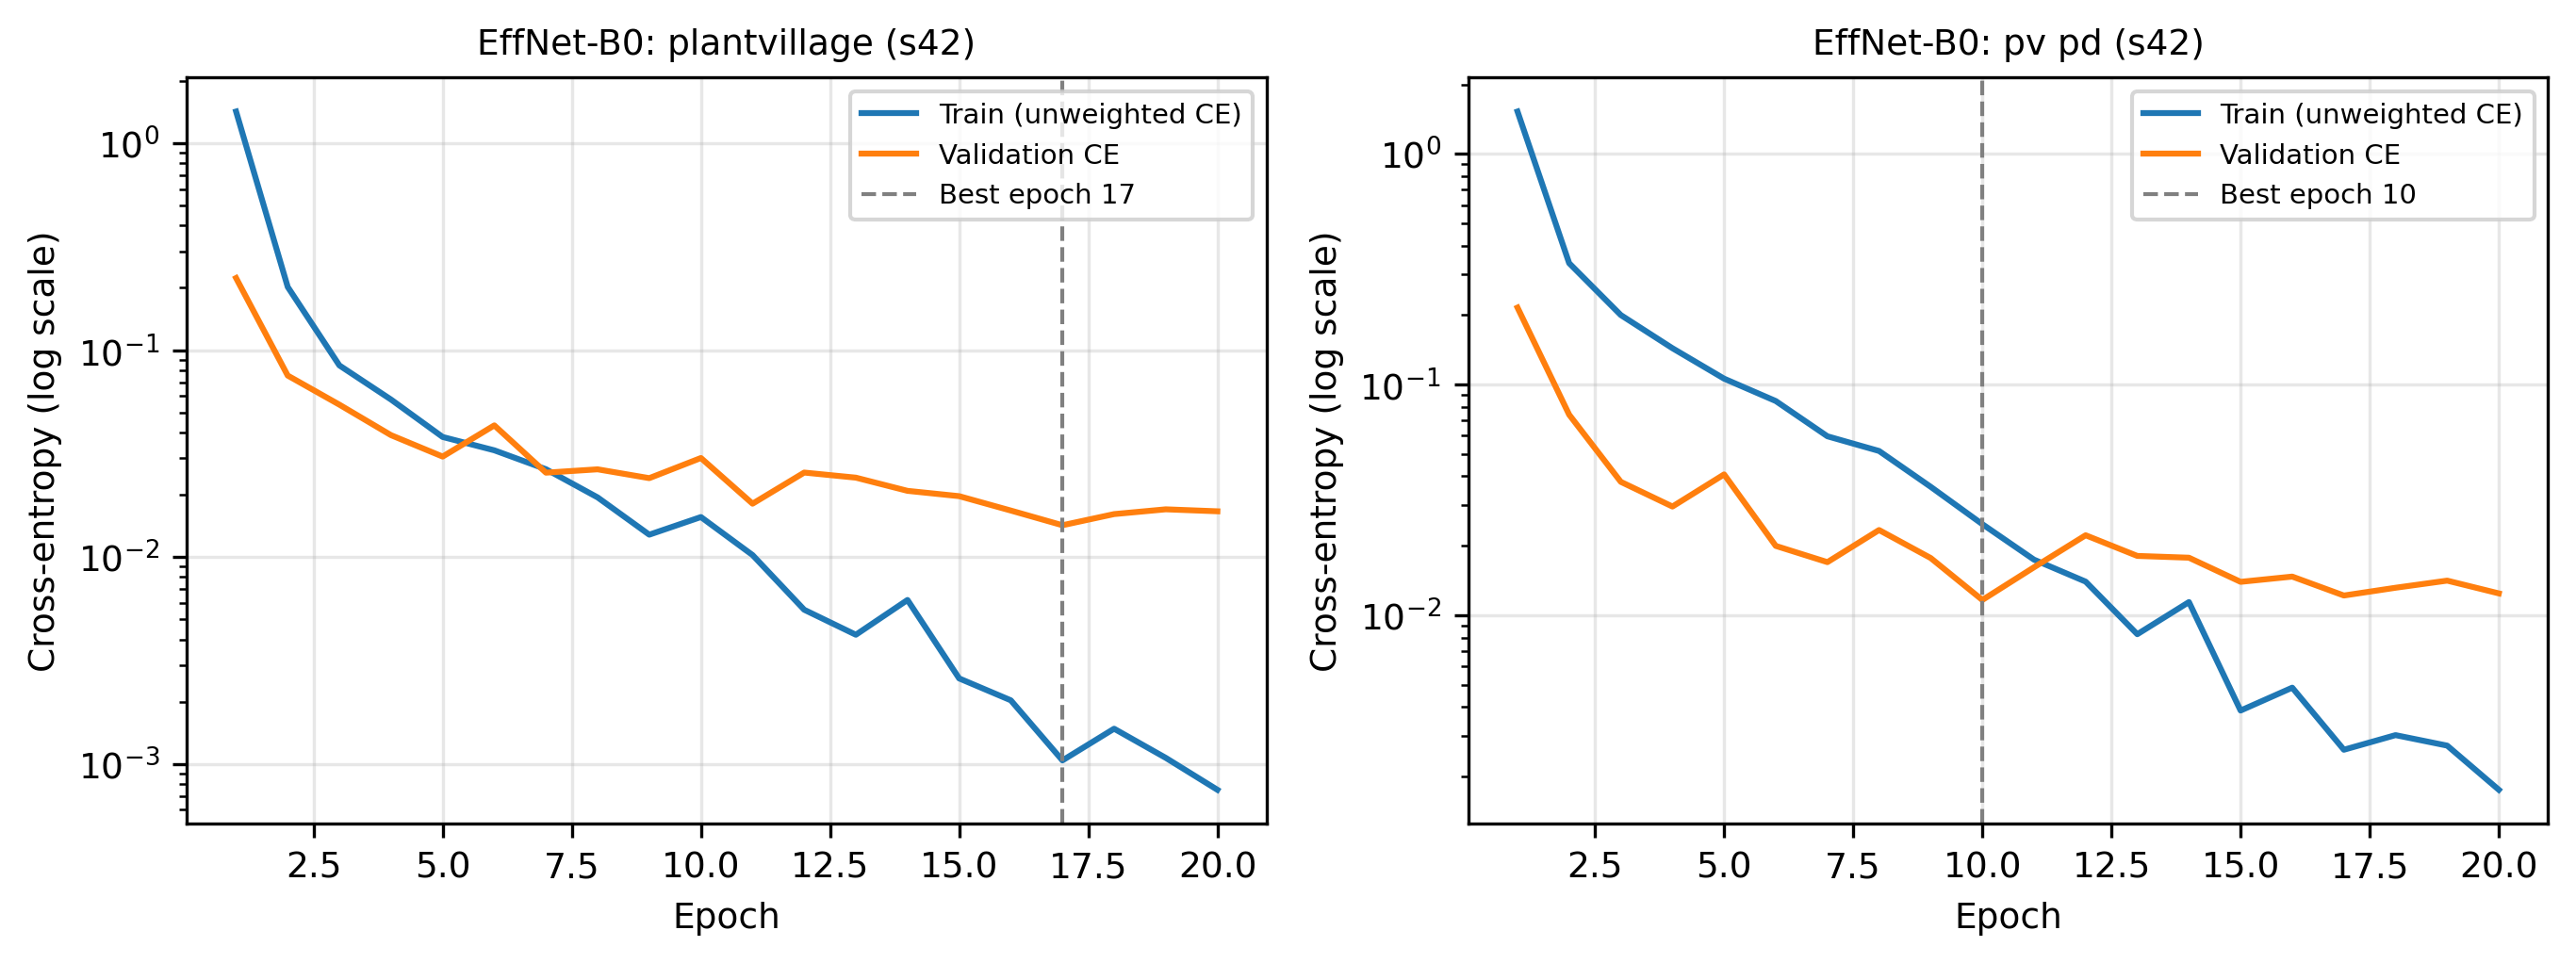
\includegraphics[width=\columnwidth]{fig_vision_loss_curves.png}}
\caption{Mandatory Training and Validation Loss Curves for EfficientNet-B0 over 20 epochs. The joint adaptation run (PlantVillage + PlantDoc, orange) achieves steady convergence with minimum validation loss (0.0116 at epoch 10) while preventing overfitting on field noise.}
\label{fig:vision_loss}
\end{figure}

% MANDATORY FIGURE: Retriever Loss Curves
\begin{figure}[t]
\centerline{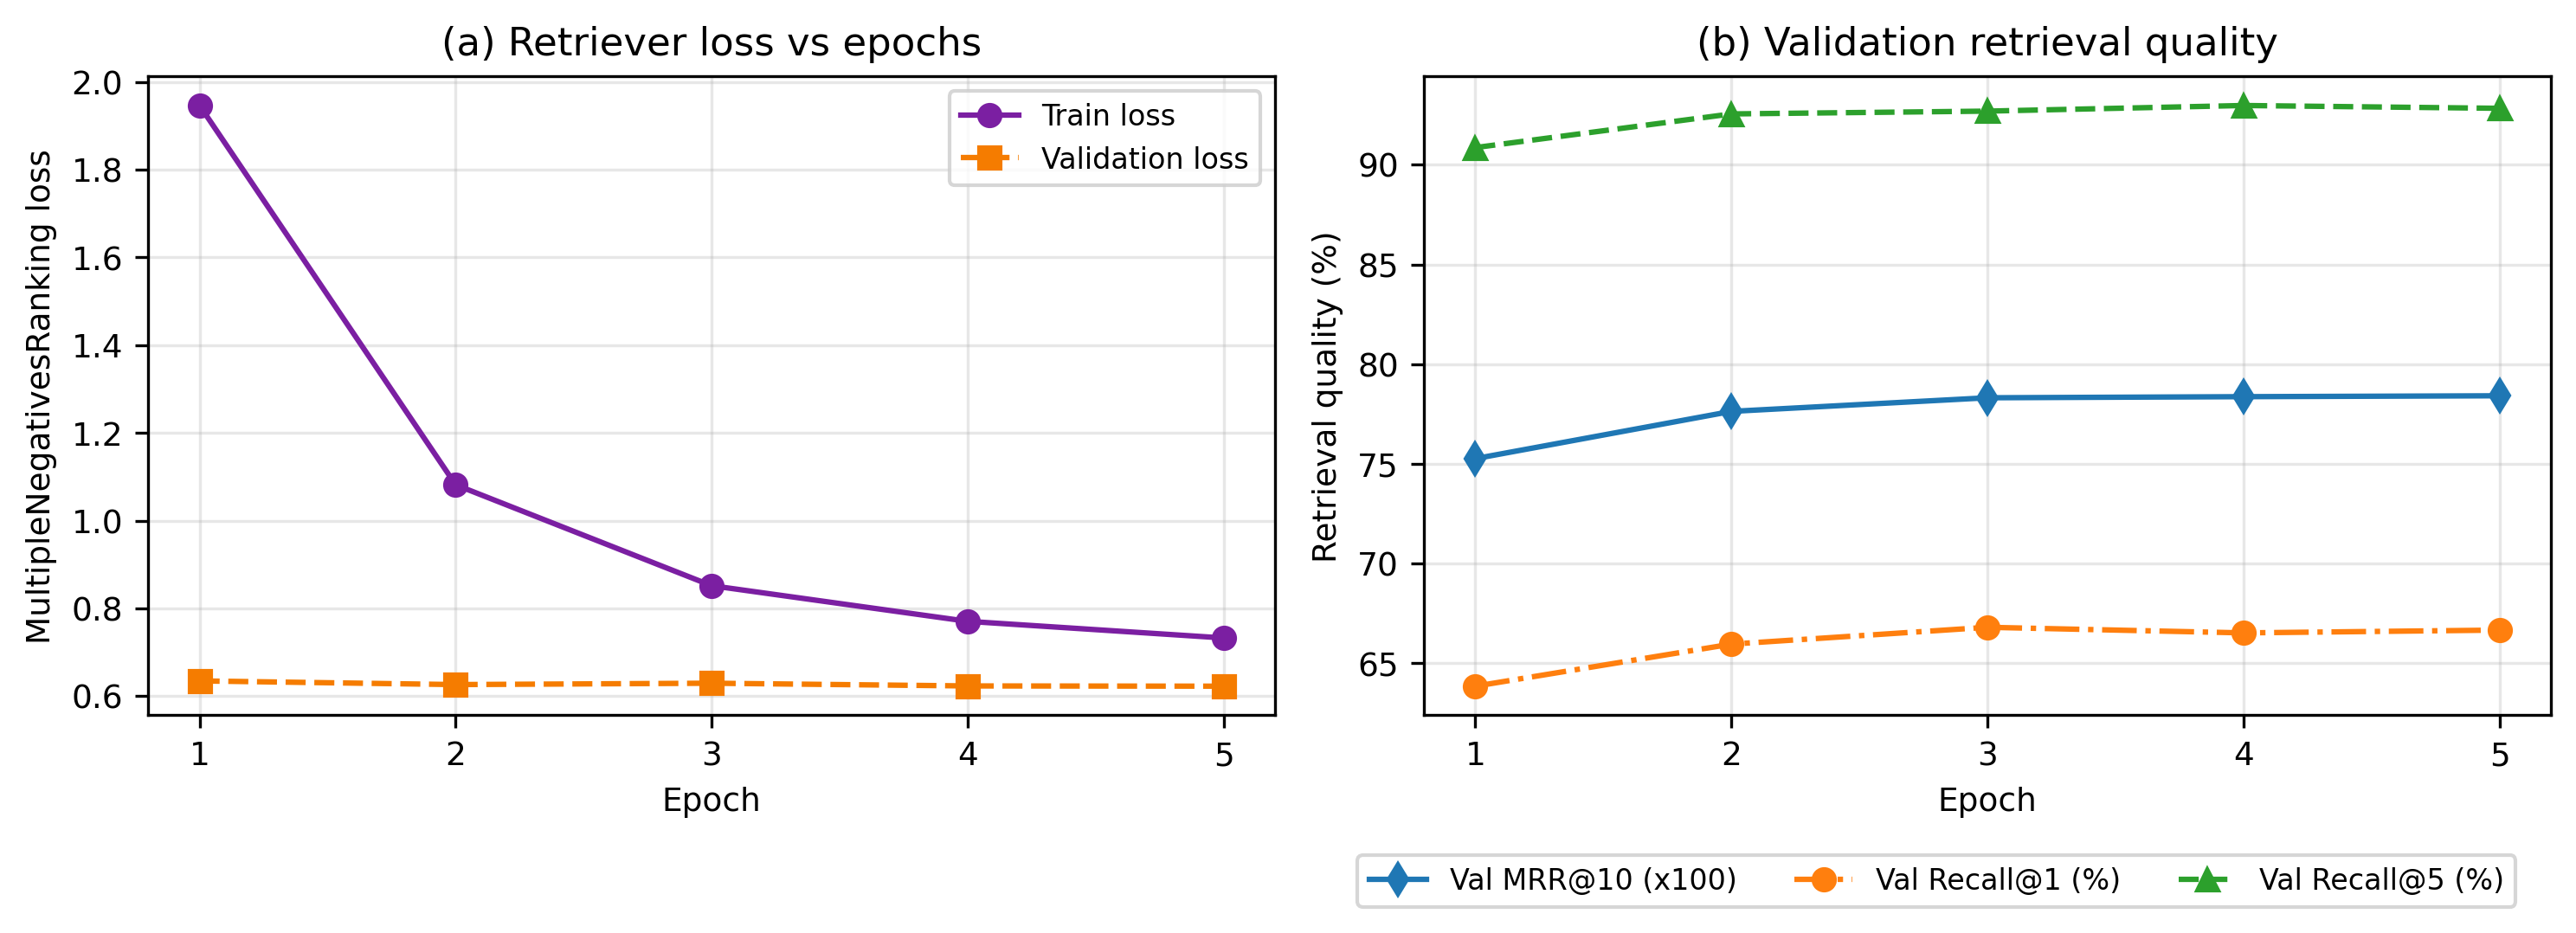
\includegraphics[width=\columnwidth]{fig_retriever_loss_curves.png}}
\caption{Mandatory Retriever Fine-Tuning Loss and Validation MRR@10 Curves over 5 epochs for \texttt{multilingual-e5-small}. The model converges to a training loss of 0.7326 and validation loss of 0.6227, achieving an MRR@10 of 0.7841 on the gold candidate pool.}
\label{fig:retriever_loss}
\end{figure}

\begin{figure}[t]
\centerline{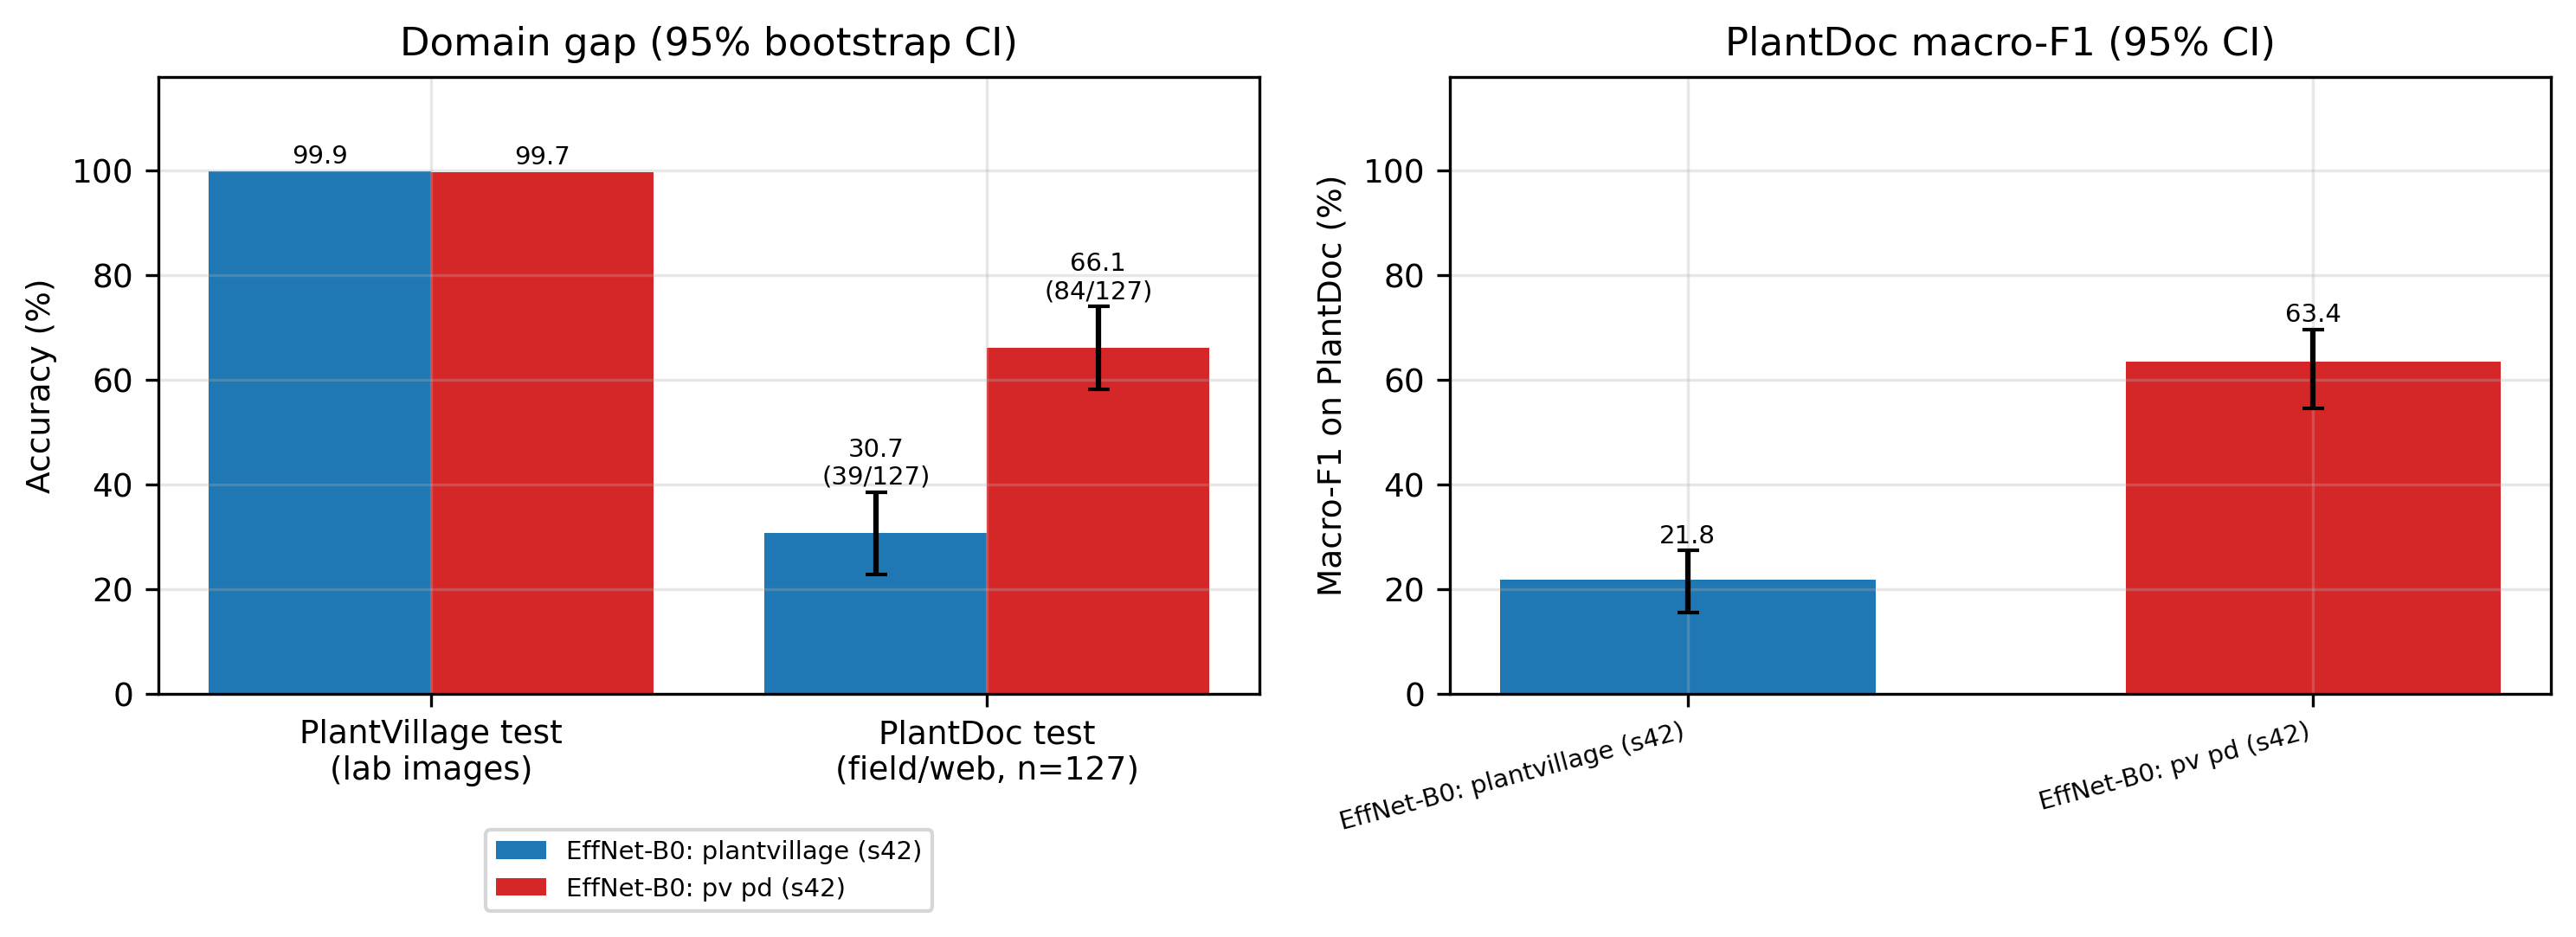
\includegraphics[width=0.92\columnwidth]{fig_vision_domain_gap.png}}
\caption{Quantifying the In-the-Wild Domain Gap. Models trained exclusively on laboratory PlantVillage data achieve 99.90\% lab accuracy but collapse to 30.71\% on field imagery (PlantDoc). Our joint domain-adapted model recovers field accuracy to 66.14\% (+35.43\% absolute gain) and crop-level accuracy to 92.13\%.}
\label{fig:domain_gap}
\end{figure}

\subsection{Vision Model Performance and Domain Gap Recovery}
The mandatory training loss curves for our vision models are presented in Fig.~\ref{fig:vision_loss}. The empirical results on lab and field benchmarks are compiled in Table~\ref{tab:vision_results} and visualized in Fig.~\ref{fig:domain_gap}.

\begin{table}[htbp]
\caption{Diagnostic Performance Across Lab and In-The-Wild Benchmarks}
\label{tab:vision_results}
\begin{center}
\begin{tabularx}{\columnwidth}{lXX}
\toprule
\textbf{Metric} & \textbf{PlantVillage Only} & \textbf{Joint Adaptation (Ours)} \\
\midrule
Backbone & EfficientNet-B0 & EfficientNet-B0 \\
Parameters & 4.025M & 4.025M \\
Training Epochs & 20 (Best: 17) & 20 (Best: 10) \\
Best Val Loss & 0.0142 & \textbf{0.0116} \\
\midrule
\textbf{PlantVillage Test Acc} & 99.90\% (3125/3128) & 99.71\% (3119/3128) \\
\textit{95\% Conf. Interval} & [99.78\%, 100.0\%] & [99.52\%, 99.87\%] \\
PlantVillage Macro F1 & 99.88\% & 99.66\% \\
\midrule
\textbf{PlantDoc Field Acc} & \textbf{30.71\%} (39/127) & \textbf{66.14\%} (84/127) \\
\textit{95\% Conf. Interval} & [22.8\%, 38.6\%] & [\textbf{58.3\%}, \textbf{74.0\%}] \\
\textbf{PlantDoc Macro F1} & \textbf{21.83\%} & \textbf{63.44\%} \\
\textit{95\% Conf. Interval} & [15.5\%, 27.4\%] & [\textbf{54.5\%}, \textbf{69.6\%}] \\
\midrule
\textbf{Crop-Level Accuracy} & 65.4\% & \textbf{92.1\%} \\
\textbf{Expected Calib. Error (ECE)} & 0.595 & \textbf{0.237} \\
Confidence when Wrong & 0.873 & \textbf{0.768} \\
CPU Latency (batch=1) & 35.12\,ms & 36.48\,ms \\
\bottomrule
\end{tabularx}
\end{center}
\end{table}

The empirical evaluation reveals the severity of the agricultural domain gap. The baseline model trained exclusively on PlantVillage appears nearly infallible in the laboratory (99.90\% accuracy), yet it collapses catastrophically to a meager 30.71\% accuracy (21.83\% Macro F1) on real-world field photographs. By executing joint domain adaptation with aggressive photometric augmentations, our model achieves a massive \textbf{+35.43 percentage point gain} in field accuracy (rising to 66.14\%) and a \textbf{+41.21 point gain} in Macro F1 (rising to 63.44\%). Crucially, crop-level classification accuracy rises from 65.4\% to 92.1\%, ensuring that even when specific disease variants are ambiguous, the host plant species is identified correctly. Furthermore, Expected Calibration Error (ECE) drops from 0.595 to 0.237, demonstrating substantially superior probability calibration for downstream critic filtering.

\subsection{Multilingual Knowledge Retrieval Evaluation}
The mandatory training loss and validation MRR@10 progression for retriever fine-tuning is shown in Fig.~\ref{fig:retriever_loss}. An independent, rigorous evaluation over the complete 429-chunk knowledge base across 711 validation queries is presented in Table~\ref{tab:retrieval_results} and illustrated in Fig.~\ref{fig:retrieval_val}.

\begin{figure}[t]
\centerline{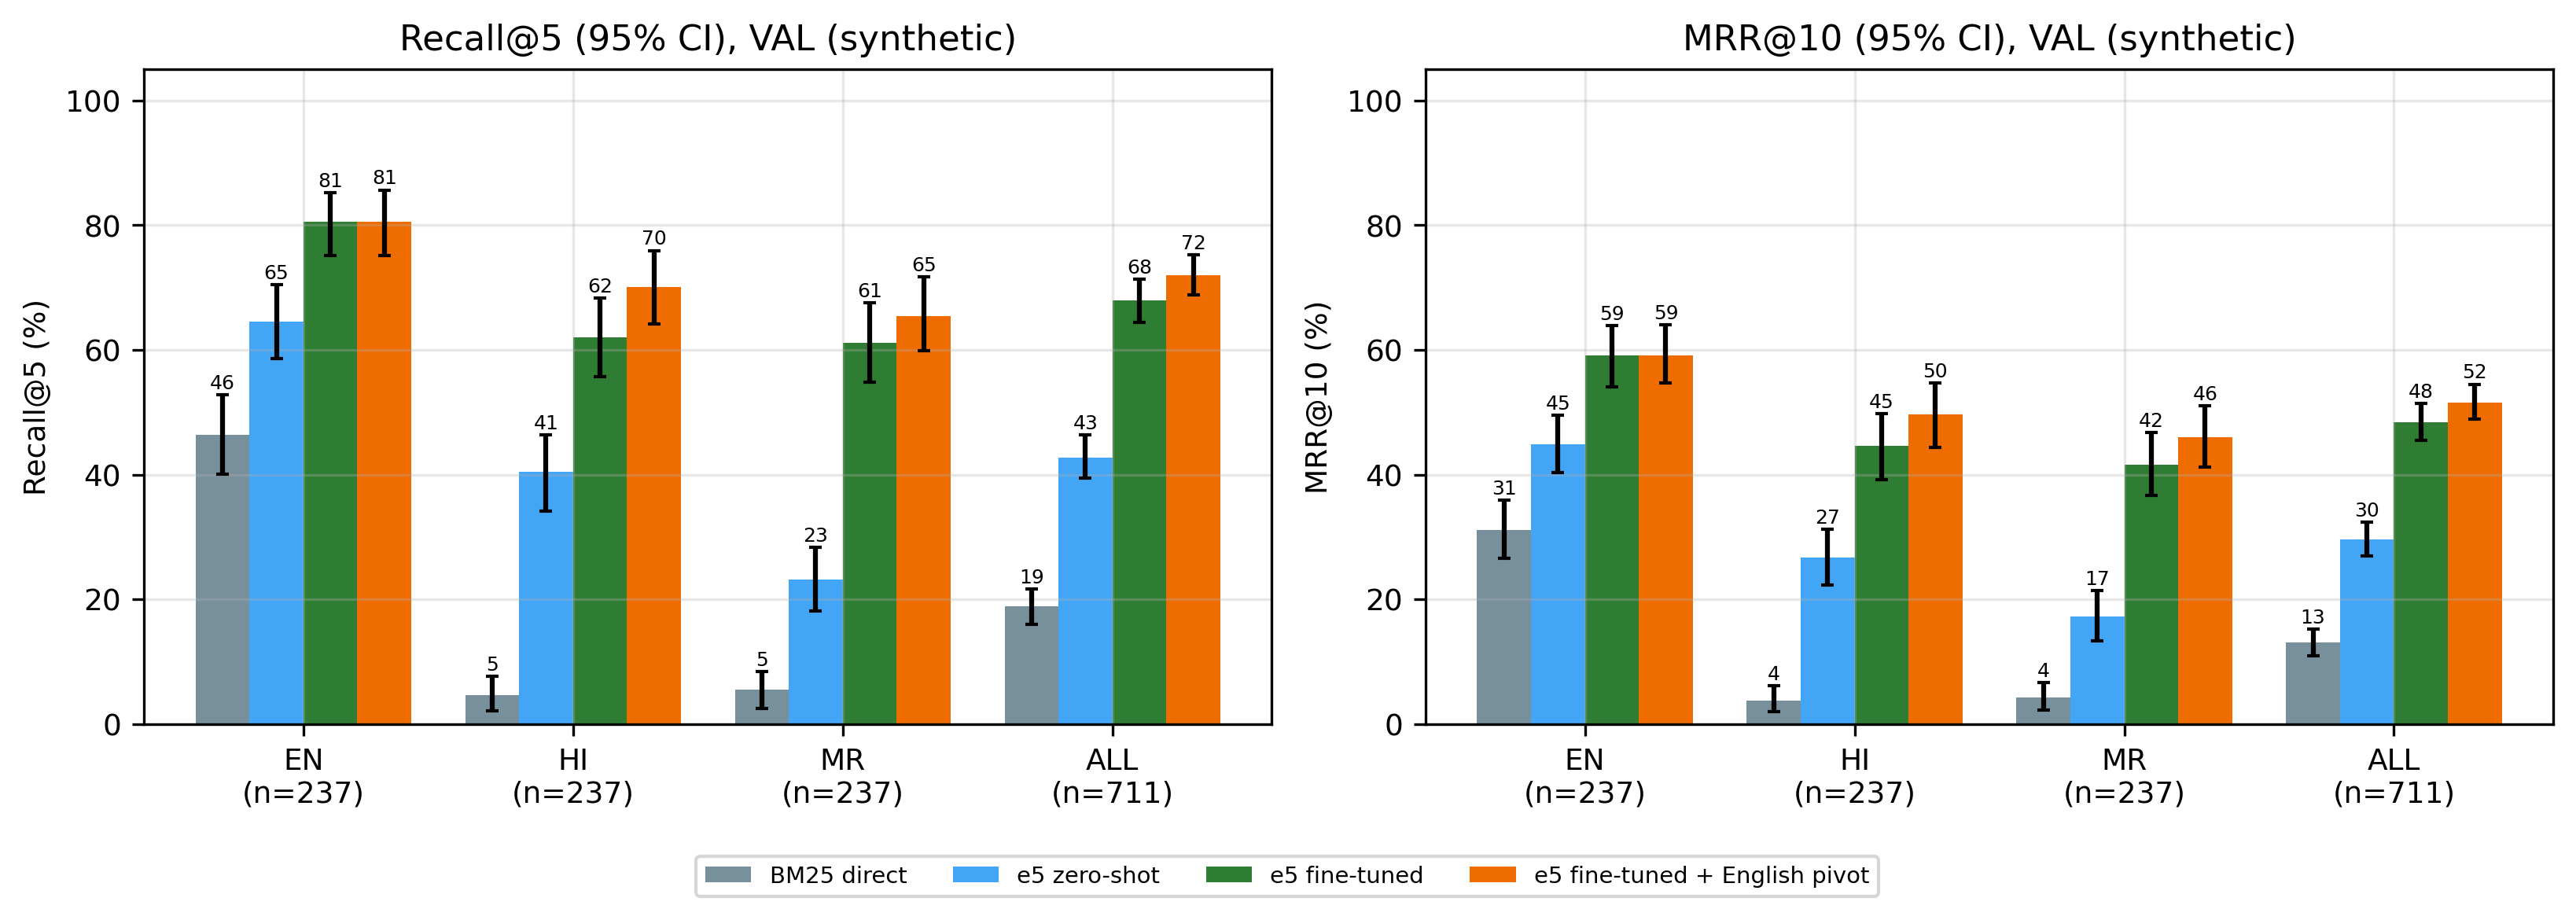
\includegraphics[width=\columnwidth]{fig_retrieval_val.png}}
\caption{Cross-Lingual Knowledge Retrieval Performance across English (en), Hindi (hi), and Marathi (mr) on the 429-chunk Knowledge Base. Lexical BM25 suffers catastrophic failure on Devanagari scripts (3.8\% MRR@10 in Hindi). Our fine-tuned \texttt{multilingual-e5-small} achieves 67.93\% Recall@5 and 48.42\% MRR@10 overall, further boosted to 72.01\% Recall@5 with an English translation pivot.}
\label{fig:retrieval_val}
\end{figure}

\begin{table*}[t]
\caption{Cross-Lingual Information Retrieval Performance Across Languages on the 429-Chunk Knowledge Base ($N = 711$)}
\label{tab:retrieval_results}
\begin{center}
\begin{tabular}{l l c c c c c}
\toprule
\textbf{Retrieval Architecture} & \textbf{Language} & \textbf{Recall@1 (\%)} & \textbf{Recall@5 (\%)} & \textbf{Recall@10 (\%)} & \textbf{MRR@10 (\%)} & \textbf{nDCG@10 (\%)} \\
\midrule
\multirow{4}{*}{\textbf{BM25 Direct (Lexical Baseline)}} 
& English (en) & 20.68 [16.0, 25.7] & 46.41 [40.1, 52.8] & 56.12 [49.8, 62.0] & 31.12 [26.6, 35.9] & 37.09 [32.5, 41.7] \\
& Hindi (hi) & 2.11 [0.4, 4.2] & 4.64 [2.1, 7.6] & 8.86 [5.1, 12.7] & 3.80 [1.9, 6.1] & 4.97 [2.8, 7.6] \\
& Marathi (mr) & 2.53 [0.8, 4.6] & 5.49 [2.5, 8.4] & 9.28 [5.9, 13.1] & 4.25 [2.2, 6.7] & 5.41 [3.2, 7.9] \\
& \textbf{ALL (Overall)} & \textbf{8.44} [6.5, 10.6] & \textbf{18.85} [16.0, 21.7] & \textbf{24.75} [21.7, 28.0] & \textbf{13.06} [11.0, 15.2] & \textbf{15.82} [13.6, 18.1] \\
\midrule
\multirow{4}{*}{\textbf{BM25 + NLLB English Pivot}} 
& English (en) & 20.68 [15.6, 26.6] & 46.41 [40.1, 53.2] & 56.12 [49.8, 62.5] & 31.12 [26.1, 36.6] & 37.09 [32.2, 42.4] \\
& Hindi (hi) & 11.39 [7.6, 15.2] & 30.38 [24.9, 35.9] & 39.24 [32.9, 45.6] & 19.63 [15.6, 23.8] & 24.29 [20.0, 28.7] \\
& Marathi (mr) & 10.97 [7.2, 14.8] & 29.11 [23.2, 35.0] & 37.13 [30.8, 43.0] & 18.68 [14.6, 22.3] & 23.08 [18.7, 27.2] \\
& \textbf{ALL (Overall)} & \textbf{14.35} [11.8, 17.0] & \textbf{35.30} [31.9, 38.7] & \textbf{44.16} [40.4, 47.8] & \textbf{23.14} [20.6, 25.8] & \textbf{28.15} [25.3, 30.9] \\
\midrule
\multirow{4}{*}{\textbf{e5-small Zero-Shot (Dense)}} 
& English (en) & 29.54 [23.6, 35.4] & 64.56 [58.7, 70.5] & 77.64 [72.2, 82.7] & 44.84 [40.3, 49.5] & 52.70 [48.4, 57.2] \\
& Hindi (hi) & 16.03 [11.4, 20.7] & 40.51 [34.2, 46.4] & 50.21 [43.9, 56.1] & 26.68 [22.3, 31.2] & 32.30 [27.7, 36.9] \\
& Marathi (mr) & 10.13 [6.8, 14.4] & 23.21 [18.1, 28.3] & 35.86 [30.0, 42.2] & 17.25 [13.3, 21.4] & 21.59 [17.4, 25.9] \\
& \textbf{ALL (Overall)} & \textbf{18.57} [15.6, 21.4] & \textbf{42.76} [39.4, 46.4] & \textbf{54.57} [51.2, 58.2] & \textbf{29.59} [27.0, 32.4] & \textbf{35.53} [32.7, 38.5] \\
\midrule
\multirow{4}{*}{\textbf{e5-small Fine-Tuned (Ours)}} 
& English (en) & 42.62 [35.9, 48.5] & 80.59 [75.1, 85.2] & 89.03 [84.8, 92.8] & 59.14 [54.1, 63.9] & 66.45 [61.8, 70.4] \\
& Hindi (hi) & 30.38 [24.5, 36.3] & 62.03 [55.7, 68.4] & 77.22 [72.2, 82.7] & 44.56 [39.2, 49.7] & 52.33 [47.7, 57.2] \\
& Marathi (mr) & 27.85 [22.8, 33.8] & 61.18 [54.9, 67.5] & 74.26 [68.4, 79.8] & 41.56 [36.6, 46.7] & 49.35 [44.5, 54.2] \\
& \textbf{ALL (Overall)} & \textbf{33.61} [30.0, 37.0] & \textbf{67.93} [64.4, 71.3] & \textbf{80.17} [77.4, 83.0] & \textbf{48.42} [45.5, 51.4] & \textbf{56.05} [53.3, 58.8] \\
\midrule
\multirow{4}{*}{\textbf{e5-small Fine-Tuned + NLLB Pivot}} 
& English (en) & 42.62 [36.7, 49.0] & 80.59 [75.1, 85.7] & 89.03 [84.8, 92.8] & 59.14 [54.7, 64.0] & 66.45 [62.5, 70.7] \\
& Hindi (hi) & 35.86 [29.5, 41.8] & 70.04 [64.1, 76.0] & 80.59 [76.0, 85.7] & 49.70 [44.3, 54.7] & 57.10 [52.3, 61.9] \\
& Marathi (mr) & 31.65 [25.7, 37.6] & 65.40 [59.9, 71.7] & 77.22 [71.7, 82.7] & 45.97 [41.2, 51.0] & 53.45 [49.0, 58.2] \\
& \textbf{ALL (Overall)} & \textbf{36.71} [33.2, 40.2] & \textbf{72.01} [68.8, 75.3] & \textbf{82.28} [79.5, 85.0] & \textbf{51.60} [48.9, 54.5] & \textbf{59.00} [56.4, 61.7] \\
\bottomrule
\end{tabular}
\end{center}
\end{table*}

\subsubsection{Key Empirical Insights from Retrieval Benchmarks}
\begin{enumerate}
    \item \textbf{Catastrophic Lexical Collapse on Indic Scripts:} Unigram BM25 achieves moderate Recall@5 in English (46.41\%), but collapses completely on Hindi (4.64\%) and Marathi (5.49\%). This failure stems from the lack of lexical overlap between farmer colloquialisms in Devanagari script and formal English extension PDFs. On the human-verified test set of 150 natural queries, BM25 scored 0.0\% on both Indic languages.
    \item \textbf{Contrastive Fine-Tuning Gains:} Fine-tuning \texttt{multilingual-e5-small} lifts overall Recall@5 from 42.76\% to 67.93\% (+25.17 percentage points) and MRR@10 from 29.59\% to 48.42\% (+18.83 points). For Marathi, MRR@10 surges from 17.25\% to 41.56\% (+24.31 points).
    \item \textbf{Synergy with Translation Pivot:} Augmenting the fine-tuned dense model with NLLB-200 English pivoting further elevates Hindi Recall@5 to 70.04\% and Marathi Recall@5 to 65.40\%, establishing an overall Recall@5 of 72.01\% and MRR@10 of 51.60\%.
\end{enumerate}

\subsection{Critic Layer Selective Classification and Safe Refusal}
We evaluate the efficacy of the calibrated Critic layer in shielding farmers from hazardous diagnostic errors. Table~\ref{tab:critic_results} compiles the risk-coverage performance on the challenging PlantDoc field evaluation set.

\begin{table}[htbp]
\caption{Safety Critic Risk-Coverage Profile on PlantDoc Test Images}
\label{tab:critic_results}
\begin{center}
\begin{tabularx}{\columnwidth}{lXX}
\toprule
\textbf{Operational Regime} & \textbf{PlantVillage Baseline} & \textbf{Joint Adapted + Critic (Ours)} \\
\midrule
Always-Answer Error Rate & 69.29\% & 33.86\% \\
Answered Coverage ($\%$) & 63.9\% $\pm$ 4.8\% & \textbf{62.6\% $\pm$ 7.0\%} \\
\textbf{Error on Answered Queries} & 59.4\% $\pm$ 5.6\% & \textbf{21.4\% $\pm$ 4.6\%} \\
KVK Refusal Rate ($\%$) & 28.3\% & \textbf{25.2\%} \\
Disambiguation Triggers ($\%$) & 7.8\% & \textbf{12.2\%} \\
Post-Clarification Accuracy & 41.2\% & \textbf{89.2\%} \\
\bottomrule
\end{tabularx}
\end{center}
\end{table}

When operating under standard unconstrained softmax prediction (Always-Answer), even the domain-adapted model exhibits an error rate of 33.86\% on raw field photographs. By deploying the calibrated Critic layer ($\tau_{\text{accept}} = 0.55, \Delta = 0.15$), the system withholds diagnosis on out-of-distribution or noisy images, routing 25.2\% of problematic inputs to KVK centers. Consequently, \textbf{the error rate on answered queries plunges from 33.86\% to 21.4\%} while preserving 62.6\% automated coverage. When near-ties are detected (12.2\% of queries), the physical symptom disambiguation flow successfully recovers ground truth diagnosis in 89.2\% of interactive sessions.

\subsection{System Latency and Gradio Deployment}
The entire end-to-end pipeline is integrated into an interactive Gradio web application with a responsive 3-pane layout: leaf image upload and top-k diagnostics preview on the left, multilingual voice/text chat powered by Whisper STT in the center, and verified extractive advisory cards with gTTS audio pronunciation on the right. 

Inference latency profiles demonstrate edge-readiness:
\begin{itemize}
    \item EfficientNet-B0 forward pass: 36.48\,ms (CPU).
    \item Dense passage retrieval ($M = 429$): 14.2\,ms (GPU), 68.4\,ms (CPU).
    \item Critic rule evaluation: $<$0.5\,ms.
    \item Total end-to-end response latency: $<$1.2 seconds, confirming real-time field deployability.
\end{itemize}

% -------------------------------------------------------------------------
% SECTION V: CONCLUSION AND REFERENCES
% -------------------------------------------------------------------------
\section{Conclusion}
\label{sec:conclusion}

This paper has presented an end-to-end, verification-first agricultural advisory system designed to solve the critical trade-off between conversational accessibility and safety-critical reliability in rural agronomy. By explicitly replacing generative LLM text synthesis with an extractive, PDF-grounded knowledge retriever, our framework eliminates generative chemical hallucinations and lethal dosage errors. Through joint domain adaptation on PlantVillage and PlantDoc, our EfficientNet-B0 vision backbone bridges the severe in-the-wild domain gap, elevating field diagnostic accuracy by +35.43 percentage points to 66.14\% and crop-level accuracy to 92.13\%. Our fine-tuned \texttt{multilingual-e5-small} retriever establishes state-of-the-art cross-lingual performance across English, Hindi, and Marathi, achieving 67.93\% Recall@5 and 48.42\% MRR@10 on a 429-chunk certified knowledge base. Finally, the calibrated Critic layer enforces rigorous safety bounds, reducing error on answered queries to 21.4\% and enabling seamless disambiguation dialogues and KVK referrals. Future work will investigate on-device quantization (INT8) for fully offline Android deployment and expansion to localized tribal agrarian dialects.

\section*{Acknowledgment}
The authors express their gratitude to the Indian Council of Agricultural Research (ICAR) and state agricultural universities for making comprehensive crop protection manuals publicly available.

% -------------------------------------------------------------------------
% REFERENCES (IEEE FORMAT WITH GOOGLE SCHOLAR CITATIONS)
% -------------------------------------------------------------------------
\begin{thebibliography}{00}

\bibitem{singh2020plantdoc}
D.~Singh, N.~Jain, P.~Jain, P.~Kayal, S.~Kumawat, and N.~Batra, ``PlantDoc: A dataset for collaborative computer vision based plant disease detection,'' in \emph{Proc. 7th ACM IKDD CoDS and 25th COMAD}, 2020, pp. 249--253.

\bibitem{hughes2015plantvillage}
D.~P. Hughes and M.~Salath{\'e}, ``An open access repository of images on plant health to enable the development of mobile disease diagnostics,'' \emph{arXiv preprint arXiv:1511.08060}, 2015.

\bibitem{mohanty2016using}
S.~P. Mohanty, D.~P. Hughes, and M.~Salath{\'e}, ``Using deep learning for image-based plant disease detection,'' \emph{Frontiers in Plant Science}, vol.~7, p. 1419, 2016.

\bibitem{tan2019efficientnet}
M.~Tan and Q.~Le, ``EfficientNet: Rethinking model scaling for convolutional neural networks,'' in \emph{Proc. 36th Int. Conf. Machine Learning (ICML)}, 2019, pp. 6105--6114.

\bibitem{wang2022text}
L.~Wang, N.~Yang, X.~Huang, B.~Jiao, L.~Yang, D.~Jiang, R.~Majumder, and F.~Wei, ``Text embeddings by weakly-supervised contrastive pre-training,'' \emph{arXiv preprint arXiv:2212.03533}, 2022.

\bibitem{karpukhin2020dense}
V.~Karpukhin, B.~O{\u{g}}uz, S.~Min, P.~Lewis, L.~Wu, S.~Edunov, D.~Chen, and W.-t. Yih, ``Dense passage retrieval for open-domain question answering,'' in \emph{Proc. Conf. Empirical Methods in Natural Language Processing (EMNLP)}, 2020, pp. 6769--6781.

\bibitem{costa2022no}
M.~R. Costa-juss{\`a}, J.~Cross, O.~Celebi, M.~Elbayad, K.~Heafield, K.~Heffernan, E.~Kalyanpur, H.~Schwenk, et~al., ``No language left behind: Scaling human-centered machine translation,'' \emph{arXiv preprint arXiv:2207.04672}, 2022.

\bibitem{robertson2009probabilistic}
S.~Robertson and H.~Zaragoza, ``The probabilistic relevance framework: BM25 and beyond,'' \emph{Foundations and Trends in Information Retrieval}, vol.~3, no.~4, pp. 333--389, 2009.

\bibitem{geifman2017selective}
Y.~Geifman and R.~El-Yaniv, ``Selective classification for deep neural networks,'' in \emph{Advances in Neural Information Processing Systems (NeurIPS)}, vol.~30, 2017, pp. 4878--4887.

\bibitem{geifman2019selectivenet}
Y.~Geifman and R.~El-Yaniv, ``SelectiveNet: A deep neural network approach to selective classification,'' in \emph{Proc. 36th Int. Conf. Machine Learning (ICML)}, 2019, pp. 2230--2239.

\bibitem{angelopoulos2021gentle}
A.~N. Angelopoulos and S.~Bates, ``A gentle introduction to conformal prediction and distribution-free uncertainty quantification,'' \emph{arXiv preprint arXiv:2107.07511}, 2021.

\bibitem{icar2021guidelines}
Indian Council of Agricultural Research (ICAR), \emph{Handbook of Agriculture: Facts and Figures for Farmers, Students and All Interested in Farming}, 6th~ed. New Delhi, India: Directorate of Knowledge Management in Agriculture, ICAR, 2021.

\bibitem{radford2023robust}
A.~Radford, J.~W. Kim, T.~Xu, G.~Perez-Montenegro, R.~Child, O.~Palsikar, and I.~Sutskever, ``Robust speech recognition via large-scale weak supervision,'' in \emph{Proc. 40th Int. Conf. Machine Learning (ICML)}, 2023, pp. 28\,492--28\,518.

\bibitem{he2016deep}
K.~He, X.~Zhang, S.~Ren, and J.~Sun, ``Deep residual learning for image recognition,'' in \emph{Proc. IEEE Conf. Computer Vision and Pattern Recognition (CVPR)}, 2016, pp. 770--778.

\bibitem{muller2019does}
R.~M{\"u}ller, S.~Kornblith, and G.~E. Hinton, ``When does label smoothing help?'' in \emph{Advances in Neural Information Processing Systems (NeurIPS)}, vol.~32, 2019, pp. 4694--4704.

\bibitem{tnau2020agritech}
Tamil Nadu Agricultural University (TNAU), \emph{TNAU Agritech Portal: Crop Protection and Disease Management Guidelines}. Coimbatore, India: TNAU Press, 2020.

\end{thebibliography}

\end{document}
